%
% A brief introduction of evolutionary algorithm, Zhang Jiadong, 2017
%

\documentclass[10pt]{beamer}

\usetheme{metropolis}
\usepackage{appendixnumberbeamer}

\usepackage{booktabs}
\usepackage[scale=2]{ccicons}
\usepackage{algorithm, algorithmic}
\usepackage{tikz}
\usepackage[BoldFont,SlantFont,CJKchecksingle]{xeCJK}
\setCJKmainfont[BoldFont=SimHei,SlantedFont=KaiTi]{SimSun}
\setCJKsansfont[BoldFont=SimHei,SlantedFont=KaiTi]{SimSun}
\setCJKmonofont[ItalicFont={Adobe Fangsong Std}]{SimSun}
\setCJKfamilyfont{zhsong}{SimSun}
\setCJKfamilyfont{zhhei}{SimHei}
\setCJKfamilyfont{zhkai}{KaiTi}
\setCJKfamilyfont{zhfs}{FangSong}

\usepackage{pgfplots}
\usepgfplotslibrary{dateplot}

\usepackage{xspace}
\newcommand{\themename}{\textbf{\textsc{metropolis}}\xspace}

\title{A brief introduction of evolutionary algorithm}
%\subtitle{A modern beamer theme}
\date{\today}
\author{XXX XXX XXX XXX XXX XXX}
\institute{College of Computer Science and Technology, Zhejiang University}
%\titlegraphic{\hfill\includegraphics[height=1.5cm]{logo.pdf}}

\begin{document}

\maketitle

\begin{frame}{Table of contents}
  \setbeamertemplate{section in toc}[sections numbered]
  \tableofcontents[hideallsubsections]
\end{frame}

\section{Introduction}

\begin{frame}[fragile]{Metropolis}

  The \themename theme is a Beamer theme with minimal visual noise
  inspired by the \href{https://github.com/hsrmbeamertheme/hsrmbeamertheme}{\textsc{hsrm} Beamer
  Theme} by Benjamin Weiss.

  Enable the theme by loading

  \begin{verbatim}    \documentclass{beamer}
    \usetheme{metropolis}\end{verbatim}

  Note, that you have to have Mozilla's \emph{Fira Sans} font and XeTeX
  installed to enjoy this wonderful typography.
\end{frame}
\begin{frame}[fragile]{Sections}
  Sections group slides of the same topic

  \begin{verbatim}    \section{Elements}\end{verbatim}

  for which \themename provides a nice progress indicator \ldots
\end{frame}

%topics

%%
% GNU courseware, XIN YUAN, 2017
%

\section{进化算法}

\frame{
\centerline{\textbf{\Huge{进化算法}}}
}

\frame{\frametitle{定义}
又叫演化计算,是模拟自然界中的生物的演化过程产生的一种群体导向的随机搜索技术和方法。

~

是一种通用的问题求解方法,具有自组织、自适应、自学习性和本质并行性等特点,
不受搜索空间限制性条件的约束,也不需要其它辅助信息。
}

\frame{\frametitle{思想}
其算法是受生物进化过程中“优胜劣汰”的自然选择机制和遗传信息的传递规律的影响,
通过程序迭代模拟这一过程,把要解决的问题看作环境,在一些可能的解组成的种群中,
通过自然演化寻求最优解。
}

\frame{\frametitle{种类}
	\begin{itemize}
		\item<1-> 遗传算法
		\item<2-> 演化策略,修改参数
		\item<3-> 演化规划,自适应响应
		\item<4-> 遗传程序设计,改变分层节点和结构链接关系
		\item<5-> 多种群协同进化,竞争和合作的动力学系统
		\item<6-> 差分进化算法,个体间竞争和合作的系统
	\end{itemize}
}

%end


%%
% GNU courseware, XIN YUAN, 2017
%

\section{免疫算法}

\frame{
\centerline{\textbf{\Huge{免疫算法}}}
}

\frame{\frametitle{定义}

\begin{block}{定义}
一种具有生成+检测 (generate and test) 的迭代过程的搜索算法。
\end{block}
}

\frame{\frametitle{思想}
生物免疫系统是一个分布式、自组织和具有动态平衡能力的自适应复杂系统。
它对外界入侵的抗原,可由分布全身的不同种类的淋巴细胞产生相应的抗体,
其目标是尽可能保证整个生物系统的基本生理功能得到正常运转。

~

具有较强模式分类能力,尤其对多模态问题的分析、处理和求解表现出较高的智能性和鲁棒性。
}

\frame{\frametitle{思想}
	\begin{itemize}
		\item<1-> 抗原和抗体
		\item<2-> 免疫疫苗
		\item<3-> 免疫算子
		\item<4-> 免疫调节
		\item<5-> 免疫记忆
		\item<6-> 抗原识别
	\end{itemize}
}

\frame{\frametitle{种类}
	\begin{itemize}
		\item<1-> 一般免疫算法
		\item<2-> 阴性选择和克隆选择算法
		\item<3-> 免疫网络学说与人工免疫网络模型
		\item<4-> 混合免疫算法
	\end{itemize}
}

\frame{\frametitle{发展}
在基于马尔科夫链的收敛性分析和非线性动力学模型等方面,
对免疫优化算法的非线性随机分析可能是未来研究的难点之一。

~

神经网络、内分泌及免疫这三大调节系统相互联系、相互补充和配合、相互制约的机理
为基于人工免疫系统的智能综合集成提供了生物学基础,
网络和智能成为免疫算法发展的不可缺少的特征,也是其重要应用领域。

~

免疫算法能增强系统的鲁棒性,在网络、智能系统和鲁棒系统中的应用。
}

%end


%%
% GNU courseware, XIN YUAN, 2017
%

\section{群聚智能}

\frame{
\centerline{\textbf{\Huge{群聚智能}}}
}

\frame{\frametitle{定义}

无智能或简单智能的主体通过任何形式的聚集协作而表现出智能行为的特性。

~

群,是一组相互之间可以进行直接或间接通信(通过改变局部环境)的主体。
}

\frame{\frametitle{思想}

源于分子自动机系统的自组织研究。
在没有集中且不提供全局模型的前提下,为寻找复杂分布式问题解决方案提供基础。
}

\frame{\frametitle{思想}
相对于传统的梯度优化算法

~

	\begin{itemize}
		\item<1-> 完全分布式处理个体间和个体环境间作用,具有自组织性;
		\item<2-> 个体间非直接,合作基于环境感知,系统可扩展和安全;
		\item<3-> 无集中控制,具有鲁棒性,个别个体失效不会影响整个问题求解;
		\item<4-> 个体智能简单,实现方便,执行时间短。
	\end{itemize}
}

\frame{\frametitle{种类}
	\begin{itemize}
		\item<1-> 蚁群(蚁狮)
		\item<2-> 鸟群(粒子群)
		\item<3-> 人工鱼群
		\item<4-> 蜂群
		\item<5-> 蛙群
		\item<6-> 萤火虫
		\item<7-> 蝙蝠群
		\item<8-> 花朵授粉
		\item<9-> 灰狼
	\end{itemize}
}

\frame{\frametitle{公式示例}

\begin{equation*}
p_{ij}^{k}(t) = \left\{
	\begin{array}{lc}
	\frac{[\tau_{ij}(t)]^{\alpha}\cdot[\eta_{ij}(t)]^{\beta}}{\sum\limits_{s\in J_{k}(i)} [\tau_{is}(t)]^{\alpha}\cdot[\eta_{is}(t)]^{\beta}}, & \mbox{如果} J \in J_{k}(i) \\
	0, & \mbox{否则}
	\end{array} \right.
\end{equation*}
}

\frame{\frametitle{定理示例}

\newtheorem{zh-thm}{定理}
\begin{zh-thm}
如果有a,b,c, 则有$a^2+b^2=c^2$。
\end{zh-thm}

\renewcommand\proofname{证明}
\begin{proof}
因为有a,b,c, 所以有$a^2+b^2=c^2$。
\end{proof}
}

\frame{\frametitle{算法示例}

\begin{algorithm}[H]
\caption{计算 $y=x^n$}\label{alg1}
\algsetup{linenosize=\tiny} \scriptsize
	\begin{algorithmic}
		\REQUIRE $n \geq 0 \vee x \neq 0$
		\ENSURE $y=x^n$
		\STATE $y \Leftarrow 1$
		\IF{$n < 0$}
			\STATE $X \Leftarrow 1 / x$
			\STATE $N \Leftarrow -n$
		\ELSE
			\STATE $X \Leftarrow x$
			\STATE $N \Leftarrow n$
		\ENDIF
		\WHILE{$N \neq 0$}
			\IF{$N$ is even}
				\STATE $X \Leftarrow X \times X$
				\STATE $N \Leftarrow N / 2$
			\ELSE[$N$ is odd]
				\STATE $y \Leftarrow y \times X$
				\STATE $N \Leftarrow N - 1$
			\ENDIF
		\ENDWHILE
	\end{algorithmic}
\end{algorithm}
}

\frame{\frametitle{流程图示例}

\tikzstyle{block}=[rectangle,draw,fill=blue!20,text width=4em,text centered,rounded corners]
\tikzstyle{huge-block}=[rectangle,draw,fill=cyan!20,text width=5em,text centered,rounded corners,minimum height=4em]
\tikzstyle{line}=[draw]
\begin{tikzpicture}[node distance=2cm, auto]
\path[use as bounding box] (-4, 0) rectangle (10, -2);
\path[line]<1-> node[huge-block](center){共享仓库};
\path[line, <->]<2-> node[block, below of=center, node distance=3cm](center-develop){开发者2}
(center)--(center-develop);
\path[line, <->]<3-> node[block, left of=center-develop, node distance=3cm](left-develop){开发者1}
(center)--(left-develop);
\path[line, <->]<4-> node[block, right of=center-develop, node distance=3cm](right-develop){开发者3}
(center)--(right-develop);
\end{tikzpicture}
}

%end


%%
% GNU courseware, XIN YUAN, 2017
%

\section{觅食算法}

\frame{
\centerline{\textbf{\Huge{觅食算法}}}
}

\frame{\frametitle{思想和种类}

{\CJKfamily{zhfs}
来自动物\textbf{高效觅食}的启发:
}

~

\begin{itemize}
	\item<2-> 布朗运动
	\item<3-> 随机游走
	\item<4-> 轻尾和重尾分布
	\item<5-> 莱维过程(L\'evy Process)
	\item<6-> 分解定理(布朗+泊松+平方可积离散鞅)
\end{itemize}
}

%end


%%
% GNU courseware, XIN YUAN, 2017
%

\section{人工神经网络}

\frame{
\centerline{\textbf{\Huge{人工神经网络}}}
}

\frame{\frametitle{定义}

人工神经网络是由大量处理单元互联组成的非线性、自适应信息处理系统。
}

\frame{\frametitle{思想}

在现代神经科学研究成果的基础上提出,试图通过模拟大脑神经网络处理、记忆信息的方式进行信息处理。

~

非线性、非局限性、非定常性、非凸性。

~

自适应、自组织、自学习。
}

\frame{\frametitle{思想}

基于逻辑符号和规则推理的专家系统,在处理直觉、非结构化信息方面有缺陷。

~

人工神经网络是连接主义的观点,是神经元相互联接而成的自适应非线性动态系统,
分为前向网络(有向无环图)和反馈网络(无向完备图)两类。

~

理论研究:MP模型、Hebb规则、感知器、适应谐振ART理论、自组织映射、认知机网络、非线性动力学。
}

\frame{\frametitle{种类}
	\begin{itemize}
		\item<1-> Hopfield
		\item<2-> 波尔兹曼机(模拟退火)
		\item<3-> 联想记忆
		\item<4-> BP
		\item<5-> 局部逼近神经网络(CMAC,RBF,B样条)
		\item<6-> 自组织SOM
		\item<7-> ART
		\item<8-> SVM
		\item<9-> 强化学习
	\end{itemize}
}

\frame{\frametitle{种类}
	\begin{itemize}
		\item<1-> 集成式网络(boosting,梯度推进机,决策树,随机森林)
		\item<2-> 量子神经网络
		\item<3-> 脉冲耦合
		\item<4-> 混沌神经网络
		\item<5-> 深度学习(卷积、循环、递归,置信网络,生成式对抗网络,迁移学习,果蝇的大脑)
	\end{itemize}
}

%end


%%
% GNU courseware, XIN YUAN, 2017
%

\section{复杂网络}

\frame{
\centerline{\textbf{\Huge{复杂网络}}}
}

\frame{\frametitle{定义}

具有自组织、自相似、吸引子、小世界、无标度中部分或全部性质的网络称为复杂网络。
}

\frame{\frametitle{思想}

互联网拓扑、社交网络、脑神经网络、基因调控网络、蛋白质调控网络、生态系统、地球演化、N体作用。
}

\frame{\frametitle{思想}
	\begin{itemize}
		\item<1-> 结构复杂:节点数巨大,结构具有多种不同特征。
		\item<2-> 网络进化:表现在节点或连接的产生与消失,网络结构不断变化。
		\item<3-> 连接多样性:节点之间的连接权重存在差异,且有可能存在方向性。
		\item<4-> 动力学复杂性:节点集可能属于非线性动力学系统,节点状态随时间发生复杂变化。
		\item<5-> 节点多样性:节点和连接可代表任何事物。
		\item<6-> 多重复杂性融合:多重复杂性相互影响,结果难以预测。
	\end{itemize}
}

\frame{\frametitle{思想}
网络的几何性质,网络的形成机制,网络演化的统计规律,网络上的模型性质,
网络的结构稳定性,网络的演化动力学机制。
}

\frame{\frametitle{种类}
	\begin{itemize}
		\item<1-> 马尔科夫场
		\item<2-> 贝叶斯网络
		\item<3-> 社交网络
		\item<4-> 视觉听觉网络
		\item<5-> 大脑生理病理网络
		\item<6-> 组分调控网络
		\item<7-> 生态系统网络(含传染病网络)
		\item<8-> 网络安全攻防
		\item<9-> 天文N体系统
	\end{itemize}
}

%end


%
% GNU courseware, XIN YUAN, 2017
%

\section{遗传程序设计}

%\frame{
%\centerline{\textbf{\Huge{遗传程序设计}}}
%}

\frame{\frametitle{背景}
\parindent=19pt	
\renewcommand{\raggedright}{\leftskip=0pt \rightskip=0pt plus 0cm}
\raggedright
自计算机出现以来,计算机科学的一个方向性目标就是让计算机自主进行程序设计,即只要告诉计算机要解决的问题,而不需要告诉它具体如何去做。遗传程序设计便是在该领域的一种尝试。

遗传程序设计最早由John Holland的遗传算法衍生而来,是一种由生物学引发的不依赖于领域的方法,它从问题需求的高层次描述中自动地产生计算机程序。

20世纪80年代以来,演化计算成为国际上诸多领域研究的热点。作为演化计算最新的分支,遗传程序设计(GP)自1990年前后提出后便成为广大学者关注的方向。
}

\frame{\frametitle{研究现状}
\parindent=19pt	
\renewcommand{\raggedright}{\leftskip=0pt \rightskip=0pt plus 0cm}
\raggedright	
目前在国外,GP在某些方面已经进入了应用性研究的阶段。在模拟与数字电路设计与分布式模糊控制方面,用GP自动设计的成果已经有了相当优良的性能。

国内对GP的研究起源于1990年前后,现在已开始成为诸多领域的研究热点。武汉大学软件工程国际重点实验室在动态系统的演化建模方面具有国际领先的水平。
}

\frame{\frametitle{定义}
\parindent=19pt	
\renewcommand{\raggedright}{\leftskip=0pt \rightskip=0pt plus 0cm}
\raggedright
遗传程序设计简称GP,是一种从生物演化过程得到灵感的自动化生成和选择计算机程序来完成用户定义的任务的技术。
}

\frame{\frametitle{原理}
\parindent=19pt	
\renewcommand{\raggedright}{\leftskip=0pt \rightskip=0pt plus 0cm}
\raggedright	
遗传程序设计借助达尔文进化论中适者生存的理论,模拟自然界生物体的自然选择和进化的过程,从产生一个随机的计算机程序群体出发,以适应值度量为衡量计算机程序解决特定问题好坏的标准,基于适应值按概率方式从群体中选出计算机程序进行复制和杂交等操作,以适当的停止准则终止循环,迭代执行其中的每一个计算机程序,在可能的计算机程序空间中寻找适应性最好的程序,最终获得对特定输入产生所要求输出的计算机程序。
}

\frame{\frametitle{对象}
\parindent=19pt	
\renewcommand{\raggedright}{\leftskip=0pt \rightskip=0pt plus 0cm}
\raggedright
与传统的数值优化算法不同,遗传程序设计的操作对象是规模和形状都能够动态变化的具有分层结构的计算机程序,从而不再局限于数值优化的范畴。
}

\frame{\frametitle{优点}
\parindent=19pt	
\renewcommand{\raggedright}{\leftskip=0pt \rightskip=0pt plus 0cm}
\raggedright	
遗传程序设计由已知的数据在适应值度量的推动下推导出其内在的未知规律即程序,避免了对求解过程的限制和先验性假设的要求。
}

\frame{\frametitle{框架}
\parindent=19pt	
\renewcommand{\raggedright}{\leftskip=0pt \rightskip=0pt plus 0cm}
\raggedright	
对程序设计问题,先产生一个不费事的有错误的解,然后再修改使它正确工作,这种做法一般要比坚持要求第一个解就完全没有缺陷的做法有效的多。遗传程序设计正是基于这样一种思想而发展起来的,它通过树的改变分层节点和结构链接关系来优化以判断是否满足终止准则,不断选择从而得到最优解。
}

\frame{\frametitle{流程图}
\begin{figure}[ht]
\centering	
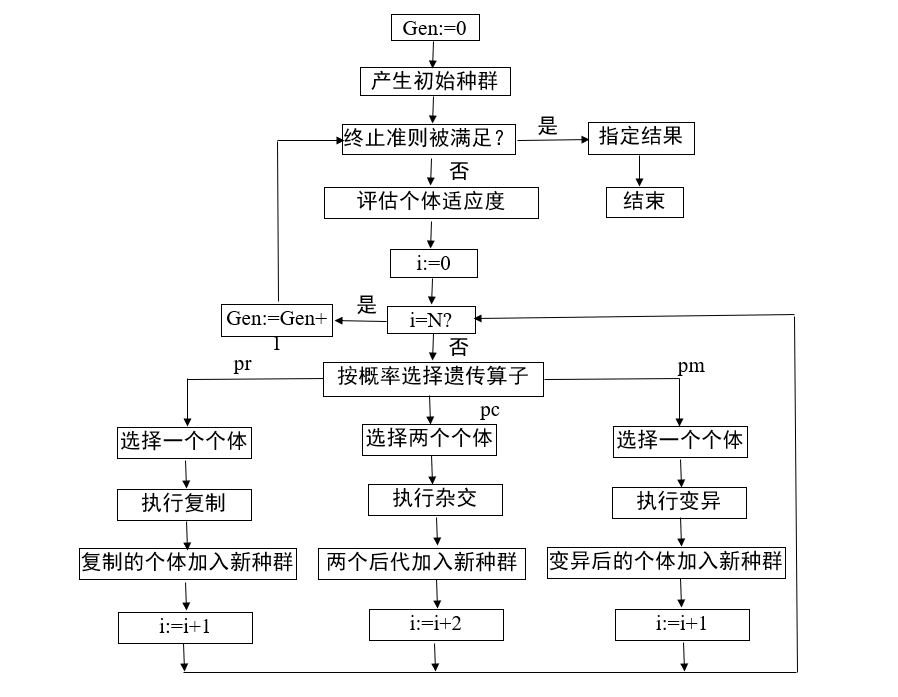
\includegraphics[scale=0.4]{../images/GP_framework.png}
\caption{遗传程序设计的流程图}
\label{fig:label}
\end{figure}
}

\frame{\frametitle{算法}
遗传程序设计的基本算法:	
	
(1)随机生成初始群体,其中个体是由表示问题的函数和终止符随机组合而成的计算机程序。
	
(2)循环执行下列各步直到满足终止准则为止:

I)运行群体中的每个计算机程序,并对其赋予适应度;

II)运行下面两个主要操作产生新的计算机程序群体:

\qquad i)把当前一代计算机程序复制成新一代计算机程序,被复制的个体依其适应度随机选定。

\qquad ii)随机选定双亲个体部位进行交叉操作产生新个体,双亲个体也依适应度随机选定。

(3)用结果标定法确定的程序被认为是运行的结果,它可能是一个正确(或近似)的问题答案。
}

\frame{\frametitle{关键}
遗传程序设计所需解决的关键问题:	
	
(1)程序的表示;

(2)程序好坏的评价标准;

(3)遗传算子的设计。
}

\frame{\frametitle{程序的表示}	
\parindent=19pt	
\renewcommand{\raggedright}{\leftskip=0pt \rightskip=0pt plus 0cm}
\raggedright
在遗传程序设计中,种群中的个体是计算机程序。为了程序表示的简单性和容易验证程序的句法,遗传程序设计用LISP语言来表示程序。

考虑一个简单的LISP程序,该程序简单地返回一个自然数n的平方:
	
>(defun square(n)(*nn))

SQUARE

下面是一个计算实数绝对值的LISP程序:

>(defun abs(x)(if(< x 0)(-x)(x)))

ABS

LISP程序的主体由类似于(*nn)和(if(< x 0)(-x)(x))的一些S-表达式所组成。

一般来说一个表示LISP程序的S-表达式通常由一些函数和端点组成。
}

\frame{\frametitle{程序的表示}	
\parindent=19pt	
\renewcommand{\raggedright}{\leftskip=0pt \rightskip=0pt plus 0cm}
\raggedright
构造LISP程序的S-表达式是以前缀表达式形式表示的。给定一个S-表达式,我们容易构造出它的语法树,而对该树进行先序遍历便可得到给定的S-表达式。
	
例如S-表达式(+12(if(> x 10)56))所对应的语法树如下图所示:

	\begin{figure}[ht]
		\centering	
		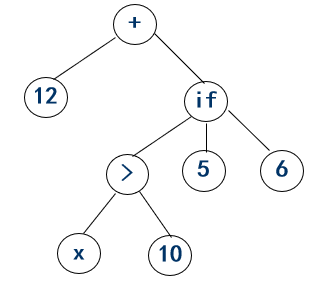
\includegraphics[scale=0.3]{../images/syntactic_tree.png}
		\caption{S-表达式的语法树}
		\label{fig:label}
	\end{figure}
	
在语法树中,树的外部结点(叶结点)分别用变量x和常量5,6,10,12来标记,这些变量和常量通常称为端点,而内部结点分别用函数+,>,IF来标记。
}

\frame{\frametitle{实现}
用遗传程序设计求解问题有以下五个基本步骤:
	\begin{itemize}		
		\item<1-> 选择端点集;
		\item<2-> 选择函数集;
		\item<3-> 确定适应函数;
		\item<4-> 确定控制参数;
		\item<5-> 确定指定结果的方法和终止程序运行的条件。
	\end{itemize}
}

\frame{\frametitle{选择端点集和函数集}
\renewcommand{\raggedright}{\leftskip=0pt \rightskip=0pt plus 0cm}
\raggedright
	\begin{itemize}		
		\item<1-> 在遗传程序设计中,计算机程序用LISP程序的语法树来表示。每一棵语法树的内部结点由一些函数构成,而叶结点由一些变量和常数构成。
		\item<2-> 对于一个给定的问题,首先要确定由所有可能求解该问题的程序所组成的程序空间S。由于LISP程序通常可以由一些简单的函数、变量和常数经过有限次运算和复合而生成。因此若要指定程序空间S,我们只要指定可以构成中程序的函数集和端点集。
		\item<3-> 函数集可以包含:
		
			<1> 算数运算 +,-,*,/等;
			
			<2> 数学函数 sin,cos,exp,log等;
			
			<3> 布尔运算 AND,OR,NOT等;
			
			<4> 条件运算 IF-THEN-ELSE等;
			
			<5> 循环运算 DO-UNTIL,FOR,WHILE等。
		\item<4-> 端点集通常由变量和常量组成。
	\end{itemize}
}

\frame{\frametitle{初始化}
	\renewcommand{\raggedright}{\leftskip=0pt \rightskip=0pt plus 0cm}
	\raggedright
	\begin{itemize}		
		\item<1-> 假设问题的端点集和函数集分别为T和F。
		\item<2-> 初始种群中的每个S-表达式,即每棵树,可按以下步骤产生:
		
			<1> 首先建立一个根结点,从函数集F中随机地选择一个函数作为根结点的标记;
		
			<2> 每当树中的一个结点被标记为函数集F中的一个函数$f$后,则为该结点建立$z(f)$个儿子结点,而每个儿子结点的标记从$C=F \bigcup T$中随机地选取;
		
			<3> 每当树中一个结点被标记为端点集T中的一个元素时,则该结点成为树的一个叶结点;
		
			<4> 如此反复进行,直到所有结点都被标记。
	\end{itemize}
}

\frame{\frametitle{初始化}
	\renewcommand{\raggedright}{\leftskip=0pt \rightskip=0pt plus 0cm}
	\raggedright
	\begin{itemize}		
		\item<1-> 假定F=\{+,-,*,/\},T=\{a,b,c,d\}。下面给出了建立一棵树结构的过程:
			\begin{figure}[ht]
			\centering	
			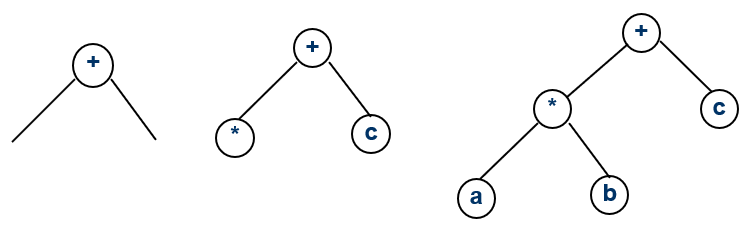
\includegraphics[scale=0.5]{../images/build_tree.png}
			\caption{语法树的构建}
			\label{fig:label}
			\end{figure}
	\end{itemize}
}

\frame{\frametitle{适应函数}
	\parindent=19pt	
	\renewcommand{\raggedright}{\leftskip=0pt \rightskip=0pt plus 0cm}
	\raggedright
	适应性函数是遗传算法和遗传程序设计得以实现的关键因素,是评价个体好坏的定量表述,决定着演化过程中群体选择复制及群体整体性的质量。

	与其它演化算法相同,在遗传程序设计中,个体的适应性函数值是判断个体的质量的唯一办法。
	
	个体适应性函数值的计算方法是问题相关的,有多种方式度量个体的适应性函数值,有些方法是明确的,有些方法是隐含的。
	
	例如,若个体是下列程序:
		\begin{figure}[ht]
		\centering	
		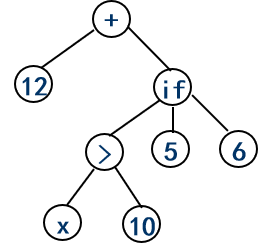
\includegraphics[scale=0.3]{../images/program.png}
		\caption{程序示例}
		\label{fig:label}
		\end{figure}
}

\frame{\frametitle{适应函数}
	\renewcommand{\raggedright}{\leftskip=0pt \rightskip=0pt plus 0cm}
	\raggedright
	评估该程序好坏的一种方法是:
	
	(1) 建立一个样本集$\{(x_{i},y_{i})|i=1,2,\Lambda,s\}$,其中$y_{i}$是当变量x取值为$x_{i}$时的期望输出;

	(2) 当$x=x_{i}(i=1,2,\Lambda,s)$时,运行该程序得到输出$z_{i}$;

     (3) 计算所得到的输出与期望输出之间的误差的绝对值之和$e=\Sigma|z_{i}-y_{i}|$;

     (4) 最后,用e作为该个体的适应性函数值。显然,适应性函数值越小,个体越好。
	
	\parindent=19pt	
	若个体是判定树,则判定树的分类准确率可以作为个体的适应性函数值。若个体是游戏策略,则游戏策略与其它策略对奕时取胜的次数可以作为个体的适应性函数值。
}

\frame{\frametitle{适应函数}
	\renewcommand{\raggedright}{\leftskip=0pt \rightskip=0pt plus 0cm}
	\raggedright
	个体适应性函数值有以下几种形式:
	
	(1) 原始适应性函数值;
	
     原始适应性函数值是以问题本身的自然术语叙述的适应性函数值度量。

     (2) 标准适应性函数值;
	
     标准适应性函数值对原始适应性函数值作简单变换,使得标准适应性函数值越小,个体越好。

     (3) 调整适应性函数值;

     调整适应性函数值$\epsilon(0,1]$。调整适应性函数值越大,个体越好。

     (4) 正规化适应性函数值。
		
	\parindent=19pt	
	正规化适应性函数值$\epsilon[0,1]$,在基于适应性函数值比例的选择策略中可直接用作选择概率。
}

\frame{\frametitle{适应函数}
	\renewcommand{\raggedright}{\leftskip=0pt \rightskip=0pt plus 0cm}
	\raggedright
	设计适应性函数,一般有以下几个步骤:
	
	(1) 原始适应性函数;
	
     按照目标函数的计算方法直接计算原始适应性函数值。

     (2) 标准化适应性函数;
	
     将得出的原始适应性函数表述为标准适应性函数。

     (3) 优化调整适应性函数;

     调整最优个体与次优个体的微小差别。

     (4) 正规化适应性函数。
		
	正规化(归一化)已优化调整的适应性函数值。
}

\frame{\frametitle{父体选择策略}
	\renewcommand{\raggedright}{\leftskip=0pt \rightskip=0pt plus 0cm}
	\raggedright	
	(1) 通常,遗传程序设计使用基于适应性函数值比例的选择策略。
	
	(2) 若种群规模在1000以上,则经常使用一种贪婪过度选择策略。
	
	(3)该策略首先将种群中的个体按适应性函数值排序,然后将种群中的个体分为两部分。第一部分包含种群$x\%$的最好个体,另一部分包含其它$(1-x\%)$的个体。当进行父体选择时,80\%的选择在第一部分中进行,20\%的选择在第二部分中进行。x的取值以来于种群规模,通常通过实验确定。
		\begin{figure}[ht]
			\centering	
			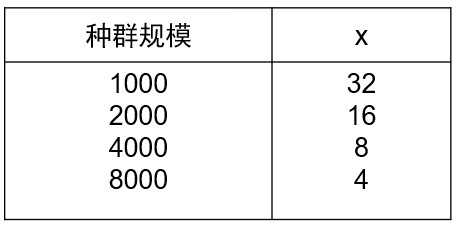
\includegraphics[scale=0.3]{../images/x_value.png}
			\caption{x的取值}
			\label{fig:label}
		\end{figure}
	
	\parindent=19pt	
	从上表可以看出,随着种群规模的增加,x不断减小,选择压力逐步增大。
}

\frame{\frametitle{遗传算子}
	\parindent=19pt
	\renewcommand{\raggedright}{\leftskip=0pt \rightskip=0pt plus 0cm}
	\raggedright	
	遗传程序设计中的遗传算子主要有复制、杂交和变异。变异算子的作用不及遗传算法中重要。
	
	(1) 复制
	
	复制算子首先按照某种基于适应性函数值比例的选择策略从种群中选择一个个体,然后将该个体不加改变地复制到下一代种群。
	
	(2) 杂交

    杂交算子分别从两个父体中随机地选择一个杂交点,然后交换父体中以杂交点为根结点的子树产生两个后代。
}

\frame{\frametitle{遗传算子}
	\renewcommand{\raggedright}{\leftskip=0pt \rightskip=0pt plus 0cm}
	\raggedright	
 	\begin{figure}[ht]
		\centering	
		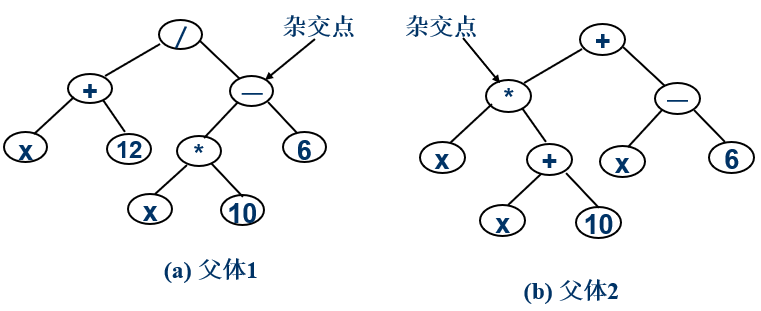
\includegraphics[scale=0.35]{../images/Hybridization1.png}
		\caption{杂交前}
		\label{fig:label}
	\end{figure}
     \begin{figure}[ht]
		\centering	
		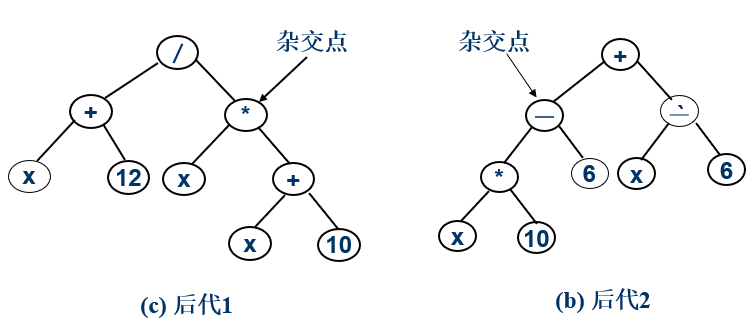
\includegraphics[scale=0.35]{../images/Hybridization2.png}
		\caption{杂交后}
		\label{fig:label}
	\end{figure}
}

\frame{\frametitle{遗传算子}
    \renewcommand{\raggedright}{\leftskip=0pt \rightskip=0pt plus 0cm}
	\raggedright	
    (3) 变异
    
    \parindent=19pt
    变异算子首先在父体中随机地选择一个结点,然后删除以该结点为根结点的子树,并在该结点处插入一个随机生成的子树。
        \begin{figure}[ht]
			\centering	
			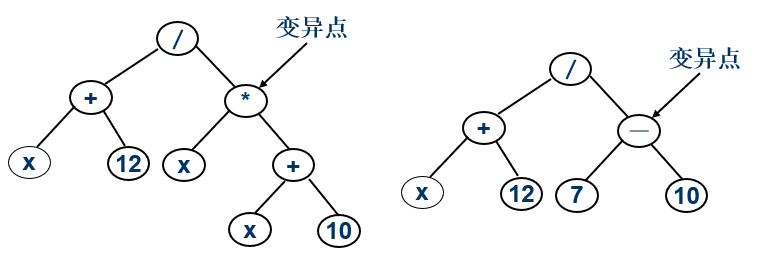
\includegraphics[scale=0.5]{../images/variation.png}
			\caption{变异}
			\label{fig:label}
		\end{figure}	
}

\frame{\frametitle{应用}
	\begin{itemize}
		\item<1-> 预测和分类:使用历史数据库来预测新事例。
		\item<2-> 符号压缩:发现各变量间的隐含关系。
		\item<3-> 机器人:控制机器人行为,使其对环境做出反应。
		\item<4-> 人工生命:用计算机模拟生物的自然进化或发现规律。
		\item<5-> 神经网络设计“设计神经网络结构、发现学习规则和相关权值,以使神经网络完成指定的任务。
		\item<6-> 图像和信号处理:图像识别、图像恢复、图像和声音的压缩等。
		\item<7-> 多Agent系统的自动设计:多个Agent协作共同处理实际问题。
		\item<8-> 游戏策略:发现一个策略打败对手。
		\item<9-> 艺术:声音、三维图像的生成、计算机动画等。
	\end{itemize}
}

\frame{\frametitle{应用实例1}
	\renewcommand{\raggedright}{\leftskip=0pt \rightskip=0pt plus 0cm}
	\raggedright	
	\begin{figure}[ht]
	\centering	
	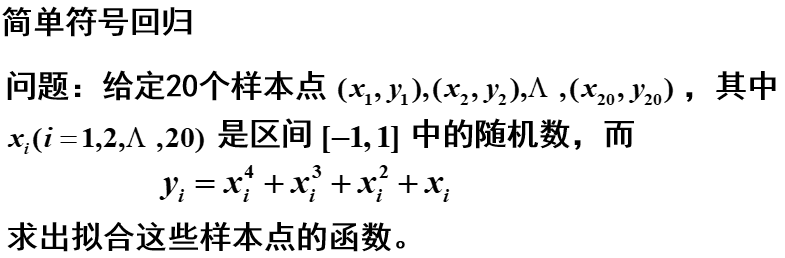
\includegraphics[scale=0.5]{../images/question.png}
	\end{figure}
}

\frame{\frametitle{应用实例1}
	\renewcommand{\raggedright}{\leftskip=0pt \rightskip=0pt plus 0cm}
	\raggedright	
	\begin{figure}[ht]
		\centering	
		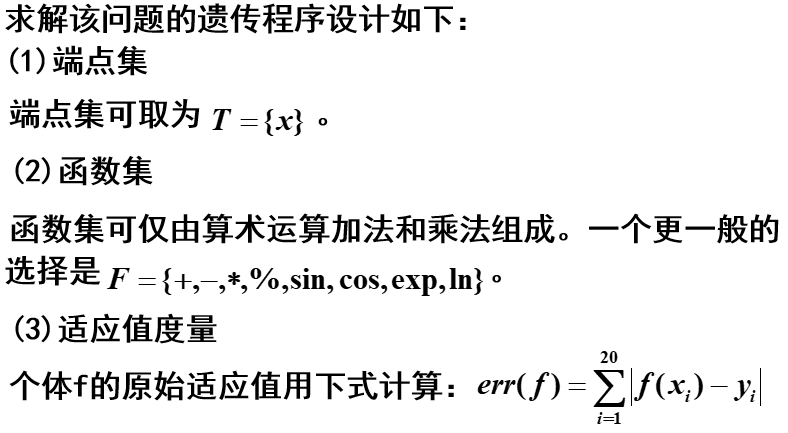
\includegraphics[scale=0.5]{../images/answer1.png}
	\end{figure}
}

\frame{\frametitle{应用实例1}
	\renewcommand{\raggedright}{\leftskip=0pt \rightskip=0pt plus 0cm}
	\raggedright	
	\begin{figure}[ht]
		\centering	
		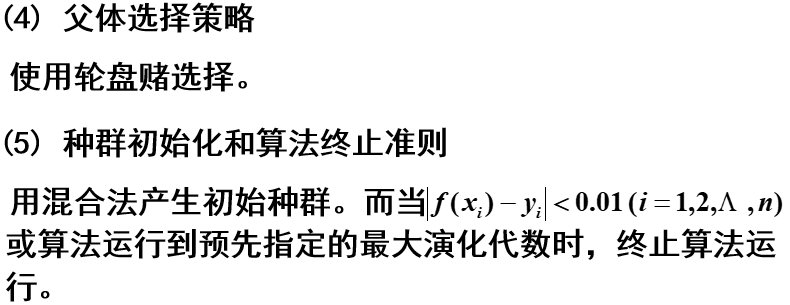
\includegraphics[scale=0.5]{../images/answer2.png}
	\end{figure}
}

\frame{\frametitle{应用实例1}
	\renewcommand{\raggedright}{\leftskip=0pt \rightskip=0pt plus 0cm}
	\raggedright	
	\begin{figure}[ht]
		\centering	
		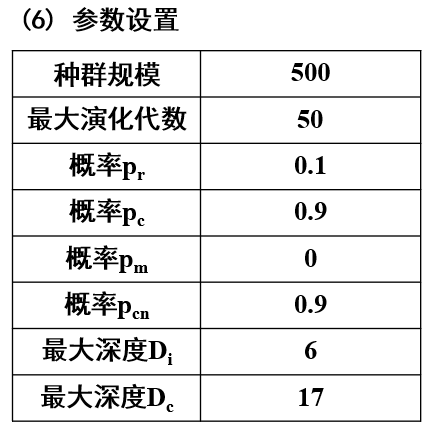
\includegraphics[scale=0.5]{../images/answer3.png}
	\end{figure}
}

\frame{\frametitle{应用实例1}
	\renewcommand{\raggedright}{\leftskip=0pt \rightskip=0pt plus 0cm}
	\raggedright	
	\begin{figure}[ht]
		\centering	
		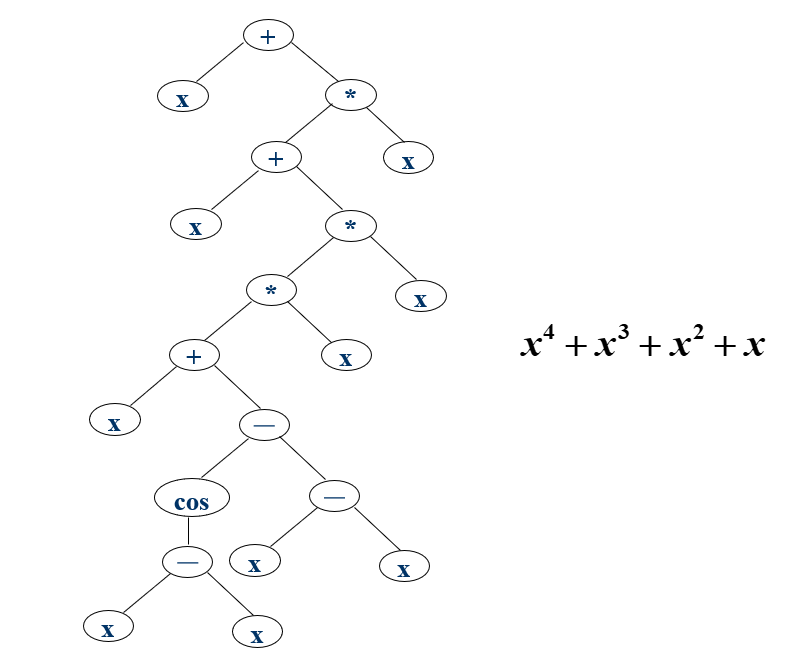
\includegraphics[scale=0.45]{../images/answer4.png}
	\end{figure}
}

\frame{\frametitle{应用实例2}
	\parindent=19pt
	\renewcommand{\raggedright}{\leftskip=0pt \rightskip=0pt plus 0cm}
	\raggedright	
	问题:给定数学表达式cos(2x),我们希望发现与cos(2x)恒等的数学表达式。
	
	将该问题视为一个符号回归问题。通过在某个区间内抽取一个随机样本,并计算给定函数在该样本的函数值,这样形成一组样本点,对所形成的样本点作符号回归。
}

\frame{\frametitle{应用实例2}
	\renewcommand{\raggedright}{\leftskip=0pt \rightskip=0pt plus 0cm}
	\raggedright	
	\begin{figure}[ht]
		\centering	
		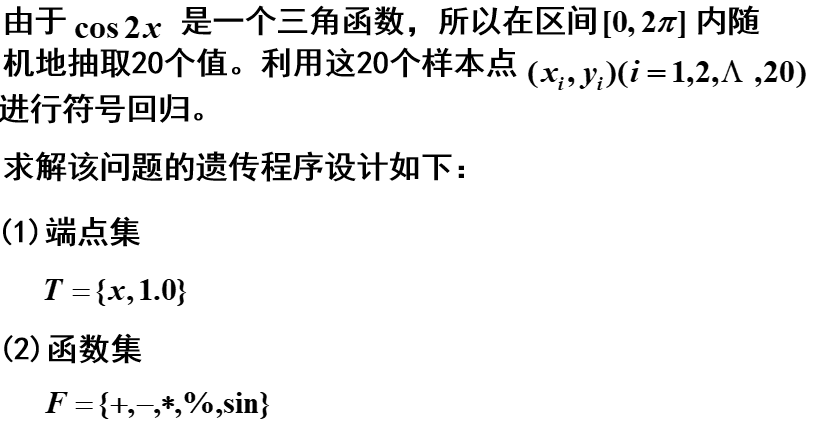
\includegraphics[scale=0.5]{../images/answer11.png}
	\end{figure}
}

\frame{\frametitle{应用实例2}
	\renewcommand{\raggedright}{\leftskip=0pt \rightskip=0pt plus 0cm}
	\raggedright	
	\begin{figure}[ht]
		\centering	
		
\includegraphics[scale=0.5]{../images/answer22.png}
	\end{figure}
}

\frame{\frametitle{应用实例2}
	\renewcommand{\raggedright}{\leftskip=0pt \rightskip=0pt plus 0cm}
	\raggedright	
	\begin{figure}[ht]
		\centering	
		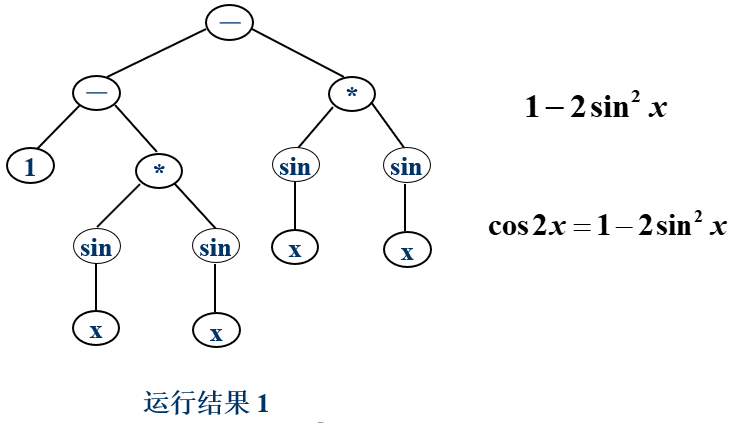
\includegraphics[scale=0.5]{../images/answer33.png}
	\end{figure}
}

\frame{\frametitle{应用实例2}
	\renewcommand{\raggedright}{\leftskip=0pt \rightskip=0pt plus 0cm}
	\raggedright	
	\begin{figure}[ht]
		\centering	
		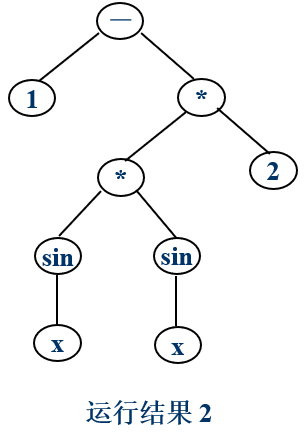
\includegraphics[scale=0.5]{../images/answer44.png}
	\end{figure}
}

\frame{\frametitle{应用实例2}
	\renewcommand{\raggedright}{\leftskip=0pt \rightskip=0pt plus 0cm}
	\raggedright	
	\begin{figure}[ht]
		\centering	
		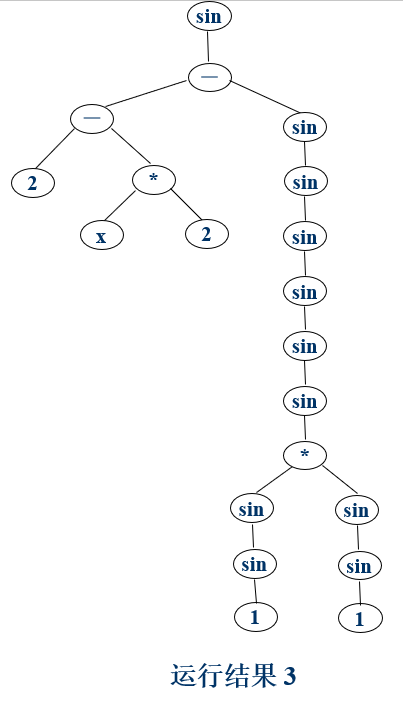
\includegraphics[scale=0.45]{../images/answer55.png}
	\end{figure}
}

\frame{\frametitle{应用实例2}
	\renewcommand{\raggedright}{\leftskip=0pt \rightskip=0pt plus 0cm}
	\raggedright	
	\begin{figure}[ht]
		\centering	
		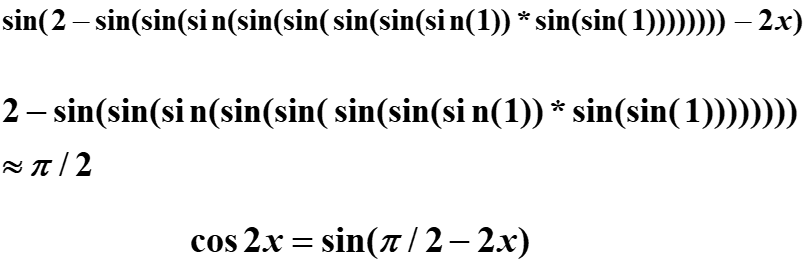
\includegraphics[scale=0.5]{../images/answer66.png}
	\end{figure}
}

\frame{\frametitle{改进}
	\parindent=19pt	
	\renewcommand{\raggedright}{\leftskip=0pt \rightskip=0pt plus 0cm}
	\raggedright
	遗传程序设计作为一种优化算法具有不需要先验性假设而可以进行全局搜索和进化最终得到最优解的特点,近年来人们在研究使用这种算法的过程中,也针对实际应用对其作了一些相应的改进:
	
	遗传程序设计主要处理树状具有分层结构的程序,在实际编程中多采用LISP语言实现。LISP语言由于缺乏统一的标准和方便的对外接口,作为一种解释语言运行速度较慢,可以采用几种具有不同数据类型的语言如PROL0G和C语言来加速程序进化的进程。
	
	传统的遗传程序设计限制少、搜索速度慢,可以用定向的非周期图(DAG)取代树和森林来存储程序群体,或针对子树进行改进,以节省程序的运行时间和空间。
	
	在算法方面,遗传程序设计可以与包括遗传算法、神经网络和模拟退火等的其他优化方法相结合,以得到更好的应用。
}

%end


%end


\section{Title formats}

\begin{frame}{Metropolis title formats}
	\themename supports 4 different title formats:
	\begin{itemize}
		\item Regular
		\item \textsc{Small caps}
		\item \textsc{all small caps}
		\item ALL CAPS
	\end{itemize}
	They can either be set at once for every title type or individually.
\end{frame}

{
    \metroset{titleformat frame=smallcaps}
\begin{frame}{Small caps}
	This frame uses the \texttt{smallcaps} title format.

	\begin{alertblock}{Potential Problems}
		Be aware that not every font supports small caps. If for example you typeset your presentation with pdfTeX and the Computer Modern Sans Serif font, every text in small caps will be typeset with the Computer Modern Serif font instead.
	\end{alertblock}
\end{frame}
}

{
\metroset{titleformat frame=allsmallcaps}
\begin{frame}{All small caps}
	This frame uses the \texttt{allsmallcaps} title format.

	\begin{alertblock}{Potential problems}
		As this title format also uses small caps you face the same problems as with the \texttt{smallcaps} title format. Additionally this format can cause some other problems. Please refer to the documentation if you consider using it.

		As a rule of thumb: just use it for plaintext-only titles.
	\end{alertblock}
\end{frame}
}

{
\metroset{titleformat frame=allcaps}
\begin{frame}{All caps}
	This frame uses the \texttt{allcaps} title format.

	\begin{alertblock}{Potential Problems}
		This title format is not as problematic as the \texttt{allsmallcaps} format, but basically suffers from the same deficiencies. So please have a look at the documentation if you want to use it.
	\end{alertblock}
\end{frame}
}

\section{Elements}

\begin{frame}[fragile]{Typography}
      \begin{verbatim}The theme provides sensible defaults to
\emph{emphasize} text, \alert{accent} parts
or show \textbf{bold} results.\end{verbatim}

  \begin{center}becomes\end{center}

  The theme provides sensible defaults to \emph{emphasize} text,
  \alert{accent} parts or show \textbf{bold} results.
\end{frame}

\begin{frame}{Font feature test}
  \begin{itemize}
    \item Regular
    \item \textit{Italic}
    \item \textsc{Small Caps}
    \item \textbf{Bold}
    \item \textbf{\textit{Bold Italic}}
    \item \textbf{\textsc{Bold Small Caps}}
    \item \texttt{Monospace}
    \item \texttt{\textit{Monospace Italic}}
    \item \texttt{\textbf{Monospace Bold}}
    \item \texttt{\textbf{\textit{Monospace Bold Italic}}}
  \end{itemize}
\end{frame}

\begin{frame}{Lists}
  \begin{columns}[T,onlytextwidth]
    \column{0.33\textwidth}
      Items
      \begin{itemize}
        \item Milk \item Eggs \item Potatoes
      \end{itemize}

    \column{0.33\textwidth}
      Enumerations
      \begin{enumerate}
        \item First, \item Second and \item Last.
      \end{enumerate}

    \column{0.33\textwidth}
      Descriptions
      \begin{description}
        \item[PowerPoint] Meeh. \item[Beamer] Yeeeha.
      \end{description}
  \end{columns}
\end{frame}
\begin{frame}{Animation}
  \begin{itemize}[<+- | alert@+>]
    \item \alert<4>{This is\only<4>{ really} important}
    \item Now this
    \item And now this
  \end{itemize}
\end{frame}
\begin{frame}{Figures}
  \begin{figure}
    \newcounter{density}
    \setcounter{density}{20}
    \begin{tikzpicture}
      \def\couleur{alerted text.fg}
      \path[coordinate] (0,0)  coordinate(A)
                  ++( 90:5cm) coordinate(B)
                  ++(0:5cm) coordinate(C)
                  ++(-90:5cm) coordinate(D);
      \draw[fill=\couleur!\thedensity] (A) -- (B) -- (C) --(D) -- cycle;
      \foreach \x in {1,...,40}{%
          \pgfmathsetcounter{density}{\thedensity+20}
          \setcounter{density}{\thedensity}
          \path[coordinate] coordinate(X) at (A){};
          \path[coordinate] (A) -- (B) coordinate[pos=.10](A)
                              -- (C) coordinate[pos=.10](B)
                              -- (D) coordinate[pos=.10](C)
                              -- (X) coordinate[pos=.10](D);
          \draw[fill=\couleur!\thedensity] (A)--(B)--(C)-- (D) -- cycle;
      }
    \end{tikzpicture}
    \caption{Rotated square from
    \href{http://www.texample.net/tikz/examples/rotated-polygons/}{texample.net}.}
  \end{figure}
\end{frame}
\begin{frame}{Tables}
  \begin{table}
    \caption{Largest cities in the world (source: Wikipedia)}
    \begin{tabular}{@{} lr @{}}
      \toprule
      City & Population\\
      \midrule
      Mexico City & 20,116,842\\
      Shanghai & 19,210,000\\
      Peking & 15,796,450\\
      Istanbul & 14,160,467\\
      \bottomrule
    \end{tabular}
  \end{table}
\end{frame}
\begin{frame}{Blocks}
  Three different block environments are pre-defined and may be styled with an
  optional background color.

  \begin{columns}[T,onlytextwidth]
    \column{0.5\textwidth}
      \begin{block}{Default}
        Block content.
      \end{block}

      \begin{alertblock}{Alert}
        Block content.
      \end{alertblock}

      \begin{exampleblock}{Example}
        Block content.
      \end{exampleblock}

    \column{0.5\textwidth}

      \metroset{block=fill}

      \begin{block}{Default}
        Block content.
      \end{block}

      \begin{alertblock}{Alert}
        Block content.
      \end{alertblock}

      \begin{exampleblock}{Example}
        Block content.
      \end{exampleblock}

  \end{columns}
\end{frame}
\begin{frame}{Math}
  \begin{equation*}
    e = \lim_{n\to \infty} \left(1 + \frac{1}{n}\right)^n
  \end{equation*}
\end{frame}
\begin{frame}{Line plots}
  \begin{figure}
    \begin{tikzpicture}
      \begin{axis}[
        mlineplot,
        width=0.9\textwidth,
        height=6cm,
      ]

        \addplot {sin(deg(x))};
        \addplot+[samples=100] {sin(deg(2*x))};

      \end{axis}
    \end{tikzpicture}
  \end{figure}
\end{frame}
\begin{frame}{Bar charts}
  \begin{figure}
    \begin{tikzpicture}
      \begin{axis}[
        mbarplot,
        xlabel={Foo},
        ylabel={Bar},
        width=0.9\textwidth,
        height=6cm,
      ]

      \addplot plot coordinates {(1, 20) (2, 25) (3, 22.4) (4, 12.4)};
      \addplot plot coordinates {(1, 18) (2, 24) (3, 23.5) (4, 13.2)};
      \addplot plot coordinates {(1, 10) (2, 19) (3, 25) (4, 15.2)};

      \legend{lorem, ipsum, dolor}

      \end{axis}
    \end{tikzpicture}
  \end{figure}
\end{frame}
\begin{frame}{Quotes}
  \begin{quote}
    Veni, Vidi, Vici
  \end{quote}
\end{frame}

{%
\setbeamertemplate{frame footer}{My custom footer}
\begin{frame}[fragile]{Frame footer}
    \themename defines a custom beamer template to add a text to the footer. It can be set via
    \begin{verbatim}\setbeamertemplate{frame footer}{My custom footer}\end{verbatim}
\end{frame}
}

\begin{frame}{References}
  Some references to showcase [allowframebreaks] \cite{knuth92,ConcreteMath,Simpson,Er01,greenwade93}
\end{frame}

\section{Conclusion}

\begin{frame}{Summary}

  Get the source of this theme and the demo presentation from

  \begin{center}\url{github.com/matze/mtheme}\end{center}

  The theme \emph{itself} is licensed under a
  \href{http://creativecommons.org/licenses/by-sa/4.0/}{Creative Commons
  Attribution-ShareAlike 4.0 International License}.

  \begin{center}\ccbysa\end{center}

\end{frame}

\begin{frame}[standout]
  Questions?
\end{frame}

\appendix

\begin{frame}[fragile]{Backup slides}
  Sometimes, it is useful to add slides at the end of your presentation to
  refer to during audience questions.

  The best way to do this is to include the \verb|appendixnumberbeamer|
  package in your preamble and call \verb|\appendix| before your backup slides.

  \themename will automatically turn off slide numbering and progress bars for
  slides in the appendix.
\end{frame}

\begin{frame}[allowframebreaks]{References}

  \bibliography{demo}
  \bibliographystyle{abbrv}

\end{frame}

\end{document}